% !TEX program = xelatex
\documentclass[10pt,a4paper]{article}

\usepackage[a4paper,top=0.66in,bottom=0.61in,left=0.76in,right=0.76in,headheight=20pt,headsep=10pt,footskip=20pt]{geometry}
\usepackage{fontspec}
\setmainfont{texgyreheros-regular.otf}[
  BoldFont=texgyreheros-bold.otf,
  ItalicFont=texgyreheros-italic.otf,
  BoldItalicFont=texgyreheros-bolditalic.otf
]
\setsansfont{texgyreheros-regular.otf}[
  BoldFont=texgyreheros-bold.otf,
  ItalicFont=texgyreheros-italic.otf,
  BoldItalicFont=texgyreheros-bolditalic.otf
]
\usepackage{microtype}
\usepackage{graphicx}
\graphicspath{{report/assets/}{assets/}}
\usepackage{booktabs}
\usepackage{tabularx}
\usepackage{array}
\usepackage{enumitem}
\usepackage{fancyhdr}
\usepackage{lastpage}
\usepackage{hyperref}
\usepackage[table]{xcolor}
\usepackage[most]{tcolorbox}
\usepackage{tikz}
\usepackage{ragged2e}

\definecolor{Navy}{HTML}{17233B}
\definecolor{Blue}{HTML}{2E74B5}
\definecolor{PaleBlue}{HTML}{EAF3FB}
\definecolor{Ink}{HTML}{18212F}
\definecolor{Muted}{HTML}{5E6B7C}
\definecolor{Light}{HTML}{F2F4F7}
\definecolor{Green}{HTML}{0A7D54}
\definecolor{Amber}{HTML}{A15C00}
\definecolor{Red}{HTML}{B42318}
\definecolor{Rule}{HTML}{D7DEE8}

\hypersetup{
  colorlinks=true,
  urlcolor=Blue,
  linkcolor=Blue,
  pdftitle={Airfoil Explorer — DRL × LBM Design Space},
  pdfauthor={Eden Golan},
  pdfsubject={AI course final-project implementation report}
}

\pagestyle{fancy}
\fancyhf{}
\fancyhead[L]{\fontsize{8}{9}\selectfont\bfseries\color{Blue}AIRFOIL EXPLORER\hspace{0.6em}\color{Muted}\mdseries· DRL × LBM DESIGN SPACE}
\fancyfoot[L]{\fontsize{7.5}{9}\selectfont\color{Muted}Submission draft · unpublished research}
\fancyfoot[R]{\fontsize{7.5}{9}\selectfont\color{Muted}\thepage\,/\,\pageref*{LastPage}}
\renewcommand{\headrulewidth}{0pt}
\renewcommand{\footrulewidth}{0pt}

\setlength{\parindent}{0pt}
\setlength{\parskip}{3.8pt}
\setlength{\tabcolsep}{5pt}
\renewcommand{\arraystretch}{1.15}
\setlist[itemize]{leftmargin=1.25em,itemsep=1.7pt,topsep=2pt,parsep=0pt}
\setlist[itemize,1]{label=\textcolor{Blue}{\small\textbullet}}

\newcommand{\eyebrow}[1]{\textcolor{Blue}{\fontsize{7.5}{8}\selectfont\bfseries\MakeUppercase{#1}}\par\vspace{2pt}}
\newcommand{\pagetitle}[3]{%
  \eyebrow{#1 / 04}%
  {\color{Blue}\fontsize{16}{18}\selectfont\bfseries #2\par}%
  \vspace{2pt}\textcolor{Rule}{\rule{\textwidth}{0.7pt}}\vspace{2pt}\par
  {\color{Muted}\fontsize{9}{11}\selectfont\itshape #3\par}\vspace{4pt}%
}
\newcommand{\sectiontitle}[1]{\vspace{3pt}{\color{Navy}\fontsize{11.2}{13}\selectfont\bfseries #1\par}\vspace{1pt}}
\newcommand{\smallbody}{\fontsize{8.55}{10.35}\selectfont}
\newcommand{\tinybody}{\fontsize{7.45}{9}\selectfont}
\newcommand{\statuspassed}{\textcolor{Green}{\bfseries Passed}}
\newcommand{\statusblocked}{\textcolor{Amber}{\bfseries Blocked}}

\newtcolorbox{callout}[1][]{
  enhanced,
  colback=PaleBlue,
  colframe=Rule,
  boxrule=0.45pt,
  arc=3mm,
  left=3mm,right=3mm,top=2.2mm,bottom=2.2mm,
  before skip=3pt,after skip=4pt,
  #1
}
\newtcolorbox{softcard}[1][]{
  enhanced,
  colback=Light,
  colframe=Rule,
  boxrule=0.4pt,
  arc=2.5mm,
  left=2.4mm,right=2.4mm,top=2mm,bottom=2mm,
  #1
}

\newcolumntype{Y}{>{\RaggedRight\arraybackslash}X}
\newcolumntype{L}[1]{>{\RaggedRight\arraybackslash}p{#1}}
\newcolumntype{C}[1]{>{\Centering\arraybackslash}p{#1}}

\begin{document}

% PAGE 1 — problem and achievement
\eyebrow{Course final project · implementation report}
{\color{Navy}\fontsize{29}{31}\selectfont\bfseries Airfoil Explorer\par}
{\color{Muted}\fontsize{13}{15}\selectfont DRL × LBM Design Space\par}
\vspace{3pt}\textcolor{Blue}{\rule{\textwidth}{1.25pt}}\vspace{4pt}

\begin{softcard}
\begin{tabularx}{\linewidth}{@{}Y Y@{}}
\eyebrow{Participant} Eden Golan & \eyebrow{Second participant} Pending — not supplied \\
\eyebrow{Date} 10 August 2026 & \eyebrow{Status} Submission draft; production evidence pending
\end{tabularx}
\end{softcard}

\sectiontitle{Problem and required achievement}
{\smallbody
The thesis workflow uses lattice Boltzmann analysis to evaluate airfoils and deep reinforcement learning to explore BP3333 geometry changes. The result set is scientifically useful but difficult to review interactively: geometry and aerodynamic coefficients must stay synchronized, while fields not approved for public release remain outside the deployed artifact.
}

\begin{callout}
{\color{Navy}\bfseries\small Defined achievement}\par\vspace{1pt}
{\smallbody A public synthetic-fixture demonstrator in which a reviewer drags geometry parameters, sees the nearest stored wing and its $C_l/C_d$ update live, and releases to snap every control to that exact row. The public contract is limited to its declared geometry, coefficient, validity, and provenance fields. The interface never predicts or interpolates aerodynamic values.}
\end{callout}

\sectiontitle{Why this is an engineering task}
{\smallbody
\begin{itemize}
  \item \textbf{Scientific consistency:} the wing and every displayed coefficient must originate from one admitted provenance row.
  \item \textbf{Interaction quality:} nearest-neighbor search must remain deterministic, fast, accessible, and stable during drag.
  \item \textbf{Publication safety:} credentials, local paths, W\&B namespace, and undeclared diagnostics remain outside the public artifact.
  \item \textbf{Operational safety:} ordinary deployment must be secret-free and fixture-only; optional live publication needs an explicit gate.
\end{itemize}
}

\sectiontitle{Safety model}
{\smallbody
The selected delivery target is a \textbf{public GitHub Pages} project site, not an authentication or email-allowlist boundary. Main/manual deployment replays only the committed fixture and needs no secret. A separate hourly/manual W\&B workflow remains disabled unless \texttt{PUBLIC\_RESEARCH\_DATA\_APPROVED=true} and an API key is present; enabling it makes the declared public contract available. URL: \href{https://edengol10.github.io/AI-final-course/}{edengol10.github.io/AI-final-course/}. References: \href{https://docs.github.com/en/pages/getting-started-with-github-pages/using-custom-workflows-with-github-pages}{GitHub Pages workflows}, \href{https://docs.github.com/en/pages/getting-started-with-github-pages/changing-the-visibility-of-your-github-pages-site}{Pages visibility}, and \href{https://docs.wandb.ai/models/track/public-api-guide}{W\&B Public API}.
}

\begin{callout}[colback=white]
{\smallbody\textbf{Repository boundary.} The thesis checkout remained a read-only scientific reference at commit \texttt{4936dea}; production code neither imports nor mutates it. All implementation lives in the separate private \texttt{AI-final-course} repository.}
\end{callout}

\newpage

% PAGE 2 — product and architecture
\pagetitle{02}{Product and architecture}{A static, credential-free client backed by validated, immutable data snapshots.}

\begin{center}
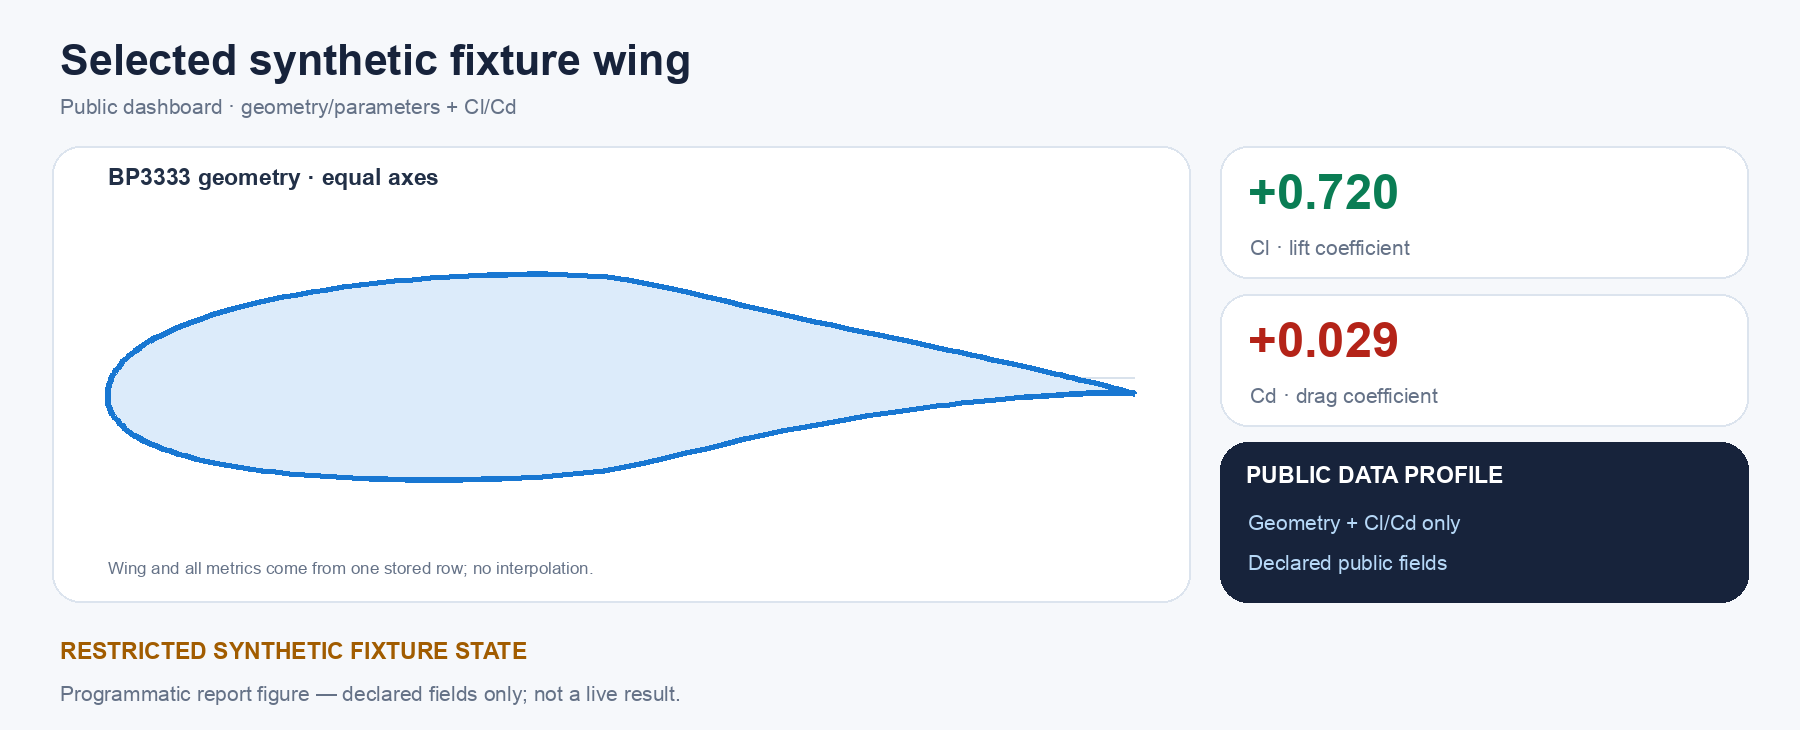
\includegraphics[width=\textwidth]{dashboard-fixture-figure.png}
\vspace{-3pt}

{\color{Muted}\fontsize{7.3}{8.5}\selectfont\itshape Figure 1. Representative UI state reconstructed from the repository's synthetic QA fixture.}
\end{center}
\vspace{2pt}

\begin{tabularx}{\textwidth}{@{}YYYY@{}}
\begin{softcard}\centering{\color{Blue}\fontsize{16}{17}\bfseries 7}\par{\tinybody unique fixture geometries}\end{softcard} &
\begin{softcard}\centering{\color{Green}\fontsize{16}{17}\bfseries 8}\par{\tinybody admitted fixture samples}\end{softcard} &
\begin{softcard}\centering{\color{Navy}\fontsize{16}{17}\bfseries 5}\par{\tinybody reviewed run identities}\end{softcard} &
\begin{softcard}\centering{\color{Amber}\fontsize{16}{17}\bfseries 6}\par{\tinybody audited fixture rejections}\end{softcard}
\end{tabularx}

\sectiontitle{Data path and trust boundary}
{\smallbody
Committed fixture $\rightarrow$ canonical JSON/SHA-256 $\rightarrow$ Vite subpath build and privacy scan $\rightarrow$ Pages artifact $\rightarrow$ public GitHub Pages $\rightarrow$ browser Zod/hash validation and Web Worker search. The optional approved W\&B path performs narrow export and admission before joining the same publication path.
}

\sectiontitle{Interaction contract}
{\smallbody
\begin{itemize}
  \item During pointer or keyboard drag, an animation-frame-throttled worker normalizes only variable parameters by authoritative BP3333 bounds and selects the exact nearest row.
  \item Ghost markers preserve requested positions; the wing, signed $C_l/C_d$ bars, and provenance preview always change together.
  \item On release, all sliders animate to the selected database vector. Stable record index breaks equal-distance ties, preventing flicker.
  \item Refresh recomputes the manifest's canonical SHA-256, then each shard's byte size and SHA-256, and validates every schema before an atomic in-memory swap. Unchanged, malformed, stale, offline, and empty states remain distinct.
\end{itemize}
}

\sectiontitle{Public data contract}
{\smallbody
The manifest's explicit \texttt{snapshotKind} is either \texttt{synthetic-fixture} or \texttt{reviewed-wandb}; the interface uses it to label fixture evidence visibly. The approved scientific outputs are BP3333 geometry/parameters and per-wing $C_l/C_d$. Minimal run/step provenance, replicate count, curvature/admission metadata, compatibility descriptors, bounds, counts, and checksums remain for auditability; W\&B entity/project names and per-row coordinate arrays are absent.
}

\newpage

% PAGE 3 — AI evidence
\pagetitle{03}{AI co-coding process and skill evidence}{AI accelerated implementation, while domain contracts and human review controlled scientific risk.}

\sectiontitle{Same-prompt before/after experiment}
\begin{callout}
{\smallbody\bfseries ``Build the W\&B-to-dashboard data refresh and nearest-wing interaction while preserving scientific validity and protecting unpublished data.''}
\end{callout}
{\smallbody
A prospective unskilled design was frozen before the custom skill was read. The identical prompt was then answered with the \emph{curate-aero-wandb-data} skill. Each output was scored 0--5 against six predeclared criteria; both artifacts and the rubric are preserved in \path{experiments/skill-comparison/}.
}

\vspace{2pt}
{\tinybody
\rowcolors{2}{white}{Light}
\begin{tabularx}{\textwidth}{@{}L{0.19\textwidth} C{0.105\textwidth} C{0.105\textwidth} Y@{}}
\rowcolor{Navy}\color{white}\bfseries Criterion & \color{white}\bfseries Without & \color{white}\bfseries With & \color{white}\bfseries Observed correction \\
Secret exposure & 4/5 & 5/5 & Exact narrow-history and exclusion boundary \\
Per-wing keys & 2/5 & 5/5 & Pinned step $C_l/C_d$ values \\
Invalid rejection & 3/5 & 5/5 & Ordered, stable reason codes \\
Physical grouping & 3/5 & 5/5 & Exact dimensions; unknowns isolated by run \\
Provenance & 4/5 & 5/5 & Minimal run/step/time tied to one metric tuple \\
Reproducibility & 3/5 & 5/5 & Authoritative bounds and deterministic representative \\
\rowcolor{PaleBlue}\bfseries Total & \bfseries 19/30 & \bfseries 30/30 & \bfseries Domain rules became testable contracts \\
\end{tabularx}
}

\sectiontitle{Material human corrections}
{\smallbody
\begin{itemize}
  \item Rejected observed-range normalization: the nearest wing would change when sample coverage changed. Fixed authoritative BP3333 bounds now define distance.
  \item Reduced the published schema to the explicitly approved geometry and coefficient fields.
  \item Removed an early per-row coordinate-array field; TypeScript reconstructs 253 geometry points from the ten parameters.
  \item Replaced an analytic reference curve with the exact BP3333 NACA2412 baseline; split unique-wing and successful-sample counts.
\end{itemize}
}

\sectiontitle{Agent split and evidence discipline}
{\smallbody
The lead established the immutable thesis boundary and integration contract. Independent data, frontend, and QA agents worked in parallel, followed by lead review. The portable project skills \texttt{curate-aero-wandb-data} and \texttt{verify-airfoil-explorer} encode future refresh and acceptance workflows. Including hosting conversion, the evidence log's conservative line items total about 24 hours 50 minutes; this report rounds down to \textbf{24 hours saved}, with scientific judgment and release approval remaining human responsibilities.
}

\begin{callout}[colback=white]
{\smallbody\textbf{Observed value of the custom skill.} The major improvement was not writing speed; it was eliminating plausible scientific errors in field choice, normalization, grouping, and replicate provenance before data crossed the publication boundary.}
\end{callout}

\newpage

% PAGE 4 — validation and limitations
\pagetitle{04}{Validation, limitations, and reflection}{Passed evidence is separated from execution-blocked work; fixture results are never presented as live research results.}

{\tinybody
\rowcolors{2}{white}{Light}
\begin{tabularx}{\textwidth}{@{}L{0.14\textwidth} Y C{0.13\textwidth}@{}}
\rowcolor{Navy}\color{white}\bfseries Area & \color{white}\bfseries Evidence & \color{white}\bfseries Status \\
Exporter & 40 Python tests; deterministic fixture, grouping, rejection, and declared profile & \statuspassed \\
Frontend & 16 tests; ESLint; strict TypeScript; production Vite build & \statuspassed \\
Geometry & 253 finite points; Python/TypeScript max error $\approx 1.2\times10^{-7}<10^{-5}$ & \statuspassed \\
Privacy & Scanner self-test and built \texttt{dist/} scan; no secret/path match & \statuspassed \\
Project skills & Both folders pass the official structural validator & \statuspassed \\
Playwright & Nine cases discovered/type-checked; loopback server denied & \statusblocked \\
Live W\&B & Client communication failed closed; fixture was not replaced & \statusblocked \\
GitHub Pages & Workflow deployed; public URL verified by HTTP smoke check & \statuspassed \\
\end{tabularx}
}

\sectiontitle{Physical validity and limits}
{\smallbody
Admission requires a finished approved run, known absolute-action schema, bounded finite actions, finite raw step $C_l/C_d$, valid geometry, and curvature ratio below one. Incompatible baseline, AoA, averaging window, or solver revision values never mix; unknown settings are isolated. Exact float32 vectors define unique geometries, while every valid replicate remains counted and traceable.

\textbf{The committed source snapshot is deliberately synthetic:} \texttt{snapshotKind=synthetic-fixture}, 8 admitted samples, and 7 geometries across five reviewed run identities. The Pages workflow rebuilds it before publication. It proves the software contract, not thesis performance. The public URL is deployed; no claim is made that live W\&B export works.
}

\sectiontitle{Reflection}
{\smallbody
\textbf{Achieved:} fixture mode demonstrates the defined interaction, one-row coefficient consistency, explicit fixture provenance, checksum-verified loading, and fail-closed refresh behavior. \textbf{Pending:} live W\&B export remains optional and unproven. AI produced substantial breadth quickly, while review kept scientific and publication decisions human-controlled. \textbf{In hindsight,} I would define the public field profile, \texttt{snapshotKind}, provenance redaction, subpath build, branch/environment protection, and deployment evidence gate before the first implementation batch.
}

\sectiontitle{Submission handoff}
\begin{tabularx}{\textwidth}{@{}Y C{1.48in}@{}}
\begin{callout}
{\smallbody\bfseries Before final submission}\par\vspace{1pt}
{\tinybody
\begin{itemize}[leftmargin=1.15em,itemsep=1pt,topsep=1pt]
  \item Insert the exact second participant name.
  \item Enable Settings $\rightarrow$ Pages $\rightarrow$ GitHub Actions.
  \item Protect \texttt{main} and require fixture CI before merge.
  \item Deploy and verify the expected URL plus public JSON paths.
  \item Confirm the artifact and UI contain only declared public fields.
  \item Run browser/mobile smoke tests and attach screenshots/video.
  \item Replace the source QR only after the Pages URL is verified.
\end{itemize}
}
\end{callout}
&
\begin{minipage}[c]{1.42in}
\centering

\includegraphics[width=0.72in]{source-repository-qr.png}\par
\vspace{1pt}{\tinybody\bfseries Private source repository}\par
\href{https://github.com/edengol10/AI-final-course}{\fontsize{6.2}{7}\selectfont github.com/edengol10}\par
\href{https://github.com/edengol10/AI-final-course}{\fontsize{6.2}{7}\selectfont AI-final-course}
\end{minipage}
\end{tabularx}

\end{document}
